\documentclass[12pt]{article}
\usepackage{fontspec}
\usepackage{polyglossia}
\setdefaultlanguage{russian}
\setmainfont[Mapping=tex-text]{CMU Serif}

\begin{document}
%% Весь этот текст можно удалить
%% ====== от сих =====
\centering {\LARGE Формальные языки}

{\Large домашнее задание на 5.03}
\bigskip

\enumerate
{
  \item
  { Построить минимальный полный ДКА для языка $L$. Доказать минимальность полученного автомата, используя \textit{критерий минимальности}: автомат минимален для данного языка $\Leftrightarrow$ все его состояния достижимы и имеют различные правые контексты. 
    \enumerate 
    {
      \item $L = \{\omega 0 0 \, | \, \omega \in \{0,1\}^*\} $
      \item $L = \{u 01101 v \, | \, u, v \in \{0,1\}^*\} $
      \item $L = \{\omega  \in \{a,b,c\}^* \, | \, |\omega|_c \neq 1 ^*\} $ (количество терминалов $c \neq 1$)
  
    }
  }
  \item Минимизировать ДКА (стартовое состояние $A$) и доказать его минимальность. 
    ~\\~{ 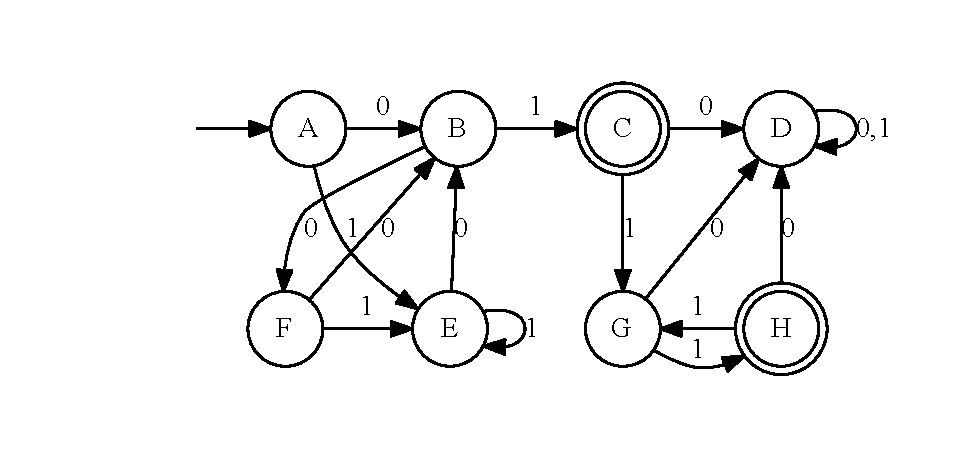
\includegraphics[width=\linewidth]{1.pdf} }
  \item На странной планете живут животные трех видов: $a, b, c$. Размножаются они тоже странно: скрещиваются особи двух разных видов, при этом родительские особи погибают, и на свет появляются 2 особи третьего вида (при скрещивании особей видов $a$ и $b$ появляются 2 особи вида $c$, родители погибают). Если на планете остаются особи только одного вида, дальнейшее размножение оказывается невозможным, что эквивалентно вымиранию. Для $n \in [3..7]$, где $n$ --- начальное количество всех животных на планете, определить, существуют ли стратегии размножения $(a)$ гарантирующие вымирание всех животных, $(b)$ гарантирующие, наоборот, что вымирание не наступит. 
}

%% ===== и до сих =====
\end{document}
